
\documentclass[11pt,a4paper,english,hyperref]{article}
\usepackage[utf8]{inputenc}

\newcommand\blattNummer{11}
\newcommand\abgabeDatum{17.5.2019}
\newcommand\ersteAufgabeNummer{1}

%%%%%%%%%%%%%%%%%%%%%%%%%%%%%%%%%%%%%%%%%%%%%%%%%%%%%%%%%%%%%%%%%%%%%%%%%% 
\usepackage{babel}
\usepackage{exscale}
\usepackage{amsmath,amsfonts,amssymb}
\usepackage[thref, amsmath, amsthm, thmmarks]{ntheorem}
\usepackage{a4wide}
\usepackage{epic,eepic}
\usepackage{graphicx} % einbinden von Grafiken mit \includegraphics
\usepackage{url}
\usepackage{mathtools}
\usepackage{etoolbox}
\usepackage[colorlinks]{hyperref}
\usepackage{enumitem}
\usepackage[capitalize]{cleveref}
\usepackage{enumitem}

\pagestyle{empty}
\parindent0em
\parskip1ex
\addtolength{\topmargin}{0cm}
\addtolength{\oddsidemargin}{0cm}
\addtolength{\textheight}{2cm}
\addtolength{\textwidth}{0cm}

% neuer Zähler für die Aufgaben
\newcounter{aufgabeNummer}
\setcounter{aufgabeNummer}{\ersteAufgabeNummer}
\addtocounter{aufgabeNummer}{-1}

% in enumerate-Umgebungen erst Kleinbuchstaben, dann kleine römische Zahlen
\renewcommand{\labelenumi}{(\alph{enumi})\,}
\renewcommand{\labelenumii}{(\roman{enumii})\,}
\setenumerate[0]{label=(\alph*)}
\crefname{enumerate}{}{}

% Stil für Definitionen, Sätze usw.
\theoremstyle{break}   % Titelzeile abgesetzt
\newtheorem{Satz}{Proposition}
\newtheorem{Lemma}{Lemma}
\newtheorem{Definition}{Definition}
\theorembodyfont{\upshape}  % normaler Font f"ur Beispiel, Aufgabe
\newtheorem{Beisiep}{Example}
\newtheorem{Aufgabe}[aufgabeNummer]{Exercise}

% Mathematische Kürzel
\newcommand\R{\mathbb{R}}
\newcommand\Q{\mathbb{Q}}
\newcommand\N{\mathbb{N}}
\newcommand\Z{\mathbb{Z}}
\renewcommand\P{\mathbb{P}}
\newcommand\T{{\mathcal T} }

\newcommand\eps{{\varepsilon}}                                  % machine precision?
\newcommand\im{{\sl i\;}}                                        % imaginary unit?
\newcommand\e{{\rm e}}                                          % Euler number
\newcommand\D{{\rm D\;}}
\DeclarePairedDelimiter\abs{\lvert}{\rvert}
\DeclarePairedDelimiter\norm{\lVert}{\rVert}
\DeclarePairedDelimiter\dotProductD{\langle}{\rangle}           % Delimiters for dot product

\DeclareMathOperator{\spann}{span}
\DeclareMathOperator{\cond}{cond}
\DeclareMathOperator{\round}{round}
\DeclareMathOperator{\supp}{supp}

\begin{document}
\parbox{0ex}{ \scalebox{.27}{  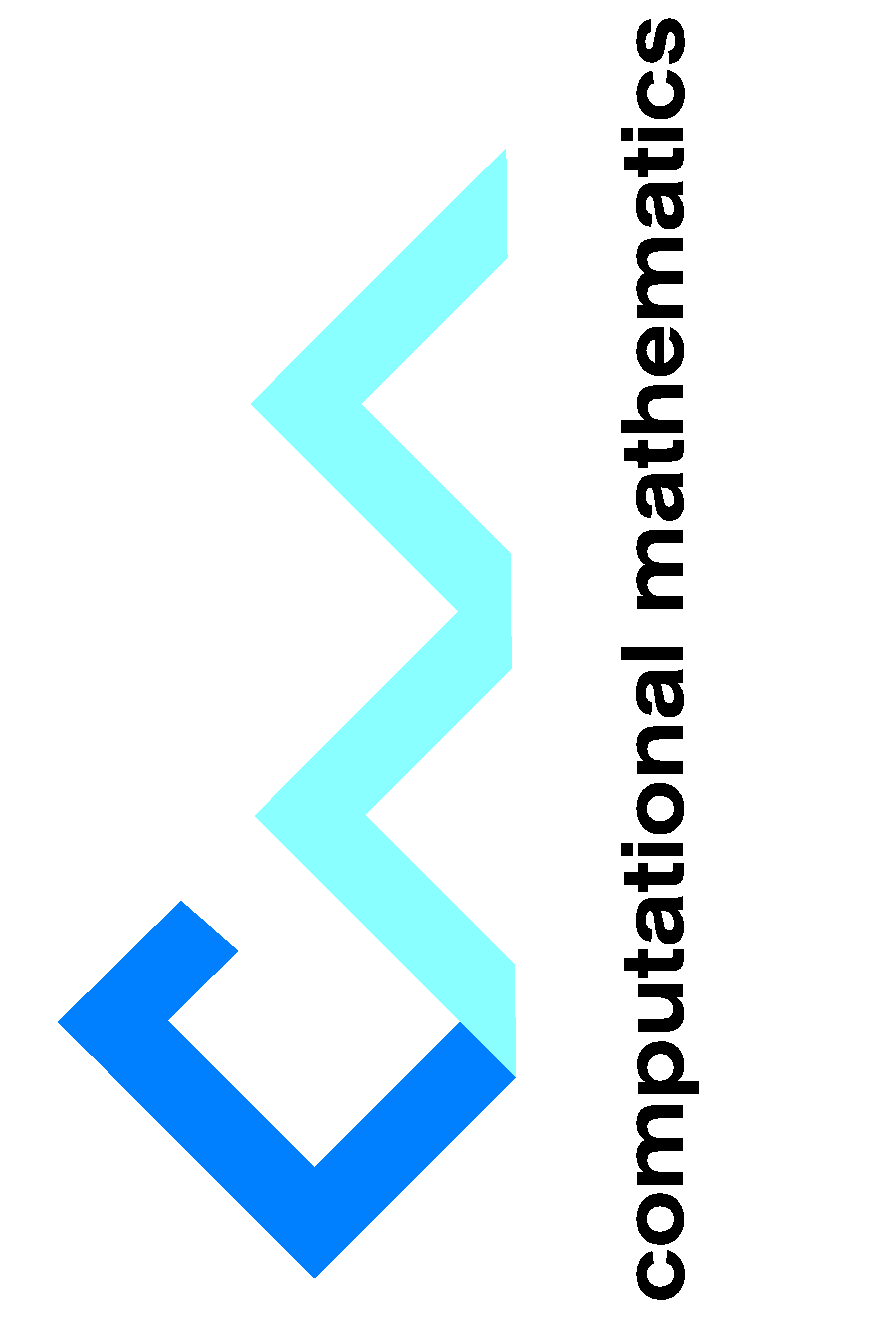
\includegraphics[width=.5\textwidth,angle=-90]{cm-logo2.eps} }   }   \\
\parbox{25ex}{
  Prof.~Dr.~S.~Sauter\\
  Institut für Mathematik\\
  Universität Zürich
  }
%
\rule[0cm]{0.cm}{.01cm}                  
\hfill  \parbox{0.6\textwidth}{
  {\sf\LARGE\bfseries Numerik I}
  {\sf\Large\bfseries \;\;--\;\; Homework \blattNummer }\\[1.5ex]
  Deadline: \abgabeDatum,\ 13:00
}
\vspace{5ex}
  
\begin{Aufgabe}[5 Points, Theoretical task]
  Prove Lemma 8.2 from the lecture notes.
\end{Aufgabe}

\begin{Aufgabe}[8 Points, Computational task]
  With reference to the lecture notes, consider the Poisson problem (8.2a).
  \begin{enumerate}
    \item Implement  a function which takes as input an integer $n$, and two functions $f,g$, and constructs the $n^2 \times n^2$ matrix $M$ and the vector $r$ of (8.6) as explained in the lecture notes ($f,g$ have the same meaning as in the lecture notes).
    \item Fix $\Omega \coloneqq [0,1]^{2}$, $f(x,y)=2\pi^2 \sin(\pi x) cos(\pi y)$ for $(x,y)\in\Omega$, $g(x,y)=\sin(\pi x) cos(\pi y)$ for $(x,y)\in\partial\Omega$. Verify that the exact solution is given by $g$ on the whole domain $\Omega$.
    \item For $8 \leq n \leq 20$ solve the resulting linear system (you can use the built-in functions of matlab and python for this task), and compute the error with respect to the exact solution; plot the error versus the number of grid points $n$ in a bilogarithmic scale.
    \item Is the error converging polynomially or exponentially? Which is the convergence rate?
    \item Produce a three-dimensional plot of the approximate solution.
  \end{enumerate}
\end{Aufgabe}

\begin{Aufgabe}[3 Points, Theoretical task]
  Prove Lemma 8.10 from the lecture notes.
\end{Aufgabe}
\end{document}